\chapter{Módszertan} 
\label{ch:methodology}

Ebben a fejezetben az alkalmazott módszertant mutatom be. Először ismertetem az alkalmazott előfeldolgozási módszereket. Ezután a tanító modellek architektúráját mutatom be. Végül pedig szót ejtek az ismertetett deep learning architektúrához tartozó hiperparaméterekről.

\section{Bemeneti adatok, előfeldolgozás}

Az OpenMIC adathalmazzal két formában kapjuk meg a bemeneti adatokat. Egyrészt elérhetőek a nyers hanganyagok .ogg formátumban. Másrészt rendelkezésre állt a VGGish nevű reprezentáció is, amelyről a \ref{subsec:VGGish}-es fejezetben írtam.

A bemeneti adatokat tanítás előtt néhány előfeldolgozási folyamaton vittem végig részben a megvalósíthatóság, részben pedig a performancianövelés érdekében. Ezekről írok a következő alfejezetekben.

\subsection{Alternatív reprezentációk kinyerése}

A .ogg fájlokból beolvasott nyers audioval való tanítás sajnos nem volt lehetséges, mivel ez egy memória szempontjából igen költséges reprezentáció, amihez a hardver eszközöm kapacitása kevésnek bizonyult. Helyette a dolgozat korábbi fejezetében bemutatott melspectogram és MFCC reprezentációkat használtam fel. Mindkét reprezentációt a beolvasott nyers hullámforma reprezentációból nyertem ki az elméleti háttér fejezetben leírt módon.

\subsection{Adathalmazok normalizálása}

Az adatok normalizálása a tanulási folyamat gyorsítására szolgál. A normalizálást úgy érjük el, hogy az adatokat arányosan a 0 és 1 értékek közé transzformáljuk. Erre egy szokásos megoldás:
\begin{equation}
x(_i) := (x(_i) - x_{\text{min}}) \/ (x_{\text{max}} - x_{\text{min}})
\end{equation}

A normalizált adathalmazon a gradiens általában hamarabb csökkenthető, ezért a tanítási folyamat rövidebb lehet. \cite{LeCun2012}

\subsection{Osztályok kiegyenlítése}

Tanító modelleknél gyakori probléma, hogy a tanulni kívánt osztályok egy része alulreprezentált. Dolgozatom multi-label osztályozása esetén két osztályról beszélhetünk: igaz (jelen van az adott hangszer) és hamis (nincs jelen az adott hangszer). Mivel sok esetben a hamis értékek jelentős többségben voltak - egyes hangszerek esetén az összes adat közel 80\%-át is kitette -, ezért a modell jó pontosságot tudott elérni csupán “hamis” predikciókkal.

Ezt elkerülendő, három megoldás jöhetett szóba:
\begin{itemize}
 \item \textbf{Alulmintavételezés (Undersampling)} - a többségi osztályokból véletlenszerűen eltávolítunk annyi elemet, hogy az osztályok kiegyensúlyozottá váljanak.
 \item \textbf{Túlmintavételezés (Oversampling)} - a kisebbségi osztályok véletlenszerű elemeit duplikáljunk addig, amíg az osztályok kiegyensúlyozottá válnak.
 \item \textbf{Adat augmentáció (Data augmentation)} - hasonlóan az oversampling technikához a kisebbségi osztály elemeit bővítjük. Ebben az esetben a meglévő elemek transzformálásával mesterségesen hozunk létre új elemeket (pl. képeknél forgatás). \cite{imbalanced}
\end{itemize}

Dolgozatom keretében az undersampling módszert alkalmaztam.

\subsection{Tanító, tesztelő, és validáló halmaz kialakítása}

Tanító modellek alkalmazásakor fontos, hogy legalább kettő, de inkább három független adathalmazzal rendelkezzünk: 
\begin{itemize}
 \item \textbf{Tanító adathalmaz (Train set)} - ebből a halmazból tanul, és ezt a halmazt látja a modellünk.
 \item \textbf{Validáló adathalmaz (Validation set)} - a tanítási lépések (epoch-ok) között ezen - a tanító halmaztól független - adathalmazon kiértékeljük modellünk működését. Ezáltal visszajelzést tudunk adni a tanítási folyamat felé, és ha szükséges, változtathatunk a hiperparamétereken. Modellünk tehát ezt a halmazt időnként látja, de nem ebből tanul.
 \item \textbf{Teszt adathalmaz (Test set)} - a tanítási folyamat végén ezen a halmazon értékeljük ki modellünk teljesítményét. Modellünk ezt a halmazt a tanítás alatt egyáltalán nem látja, és ezáltal nem is tud tanulni belőle. Ezzel a függetlenséggel biztosítjuk a kiértékelés torzítatlanságát. \cite{traintestvalid}
\end{itemize}

Bevett szokás, hogy az adathalmazunkat véletlenszerűen, körülbelül 60\%-20\%-20\% arányban felosztjuk a fent említett három diszjunkt halmazra úgy, hogy a nagyobb részt a tanító halmaz kapja. \cite{traintestvalid} Dolgozatom során én is ezt az elvet követtem.

\section{Architektúra}

A következő alfejezetekben a különböző tanító modell kísérletek architektúráját mutatom be.

\subsection{Hagyományos machine learning (Modeling Baseline)}

Az OpenMIC dataset megalkotói bemutattak egy példa modellt, amely egy véletlen erdő osztályozó (random forest classifier). \cite{humphrey2018openmic} Ez egy hagyományos gépi tanulási algoritmus. Az osztályozó 100 eldöntési fából áll, a maximális mélysége 8. Ez szolgált munkám kiinduló pontjaként. A továbbiakban Modeling Baseline elnevezéssel hivatkozok rá.

A Modeling Baseline futtatását alapvetően a VGGish reprezentációra implementálták. Dolgozatom keretében megvalósítottam ugyanennek az osztályozónak a melspectogram, illetve MFCC reprezentációkon való tanítását is. Ezáltal minden reprezentációra kaptam egy viszonyítási alapot.

\subsection{Deep CNN}

Az első mély tanulási megközelítésem a VGG-16 \cite{vgg} architektúrához hasonló mély konvolúciós neuronháló megvalósítása. Ennek megfelelően Deep CNN néven fogok rá hivatkozni a továbbiakban. A VGG-16 egy 2014-ben bemutatott architektúra, amelyet 224x224 méretű RGB képek tanítására hoztak létre. Több tanulmány is azt állítja, hogy az ehhez hasonló mély konvolúciós hálók hangok tanítására is alkalmasak lehetnek (például \cite{choi2017tutorial}). Erre az állításra az intuíció pedig az lehet, hogy a hangok különböző kétdimenziós reprezentációi képek, melyekben a mély konvolúciós hálók mintákat, összefüggéseket tudnak keresni.

\begin{figure}[H]
  \centering
  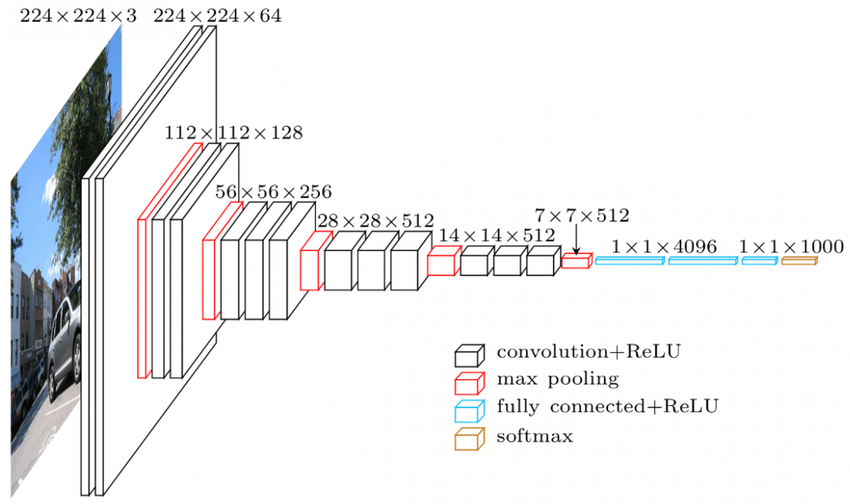
\includegraphics[width=\textwidth, height=8cm]{vgg.png}
  \caption{VGG-16 neurális háló architektúrája, forrás: \cite{loukadakis2018}}
\end{figure}

Az architektúra a következő elemekből épül fel:

\begin{itemize}
 \item konvolúciós rétegek, ReLU aktivációs függvénnyel
 \item max-pooling rétegek
 \item opcionálisan dropout rétegek
 \item flattening réteg
 \item teljesen kapcsolt rétegek, ReLU aktivációs függvénnyel
 \item teljesen kapcsolt utolsó réteg, szigmoid aktivációs függvénnyel
\end{itemize}

A bemenetet először két konvolúciós rétegnek adjuk át. Ezt követi egy max-pooling réteg, majd esetleg a nagyobb random-faktor érdekében egy dropout réteg. Ezután ugyanilyen sorrendben még háromszor-négyszer (attól függően, milyen mély architektúrát szeretnénk megvalósítani) hozzáfűzzük ezeket a rétegeket az előző kimenetéhez. Ahogy a konvulúciós rétegek zsugorodnak a max-poolingok hatásaként, úgy egyre több szűrővel érdemes ellátni őket. A következő egy flattening réteg, amely lehetőséget biztosít arra, hogy teljesen kapcsolt rétegeket csatoljunk utána. Dropout rétegeket itt is alkalmazhatunk. Az utolsó teljesen kapcsolt réteghez szigmoid aktivációs függvény tartozik, hogy 0 és 1 közötti értékeket kapjunk a kimenetre. Ebből nyerjük ki a végleges igaz-hamis értékeket.

Erre az architektúrára csak a melspectogram reprezentációt lehetett ráilleszteni. A VGGish 10 és az MFCC 20 méretű dimenziója a konvolúciók és összevonások következtében nulla alá redukálódott volna, ami nem lehetséges. Ezért ezen architektúrával a kísérlezetést abbahagytam, ezt egy későbbi kutatás során lehetne folytatni.

\begin{table}[H]
	\centering
	\begin{tabular}{ | c | c |}
		\hline
		\textbf{Réteg} & \textbf{Melspec}  \\
		\hline \hline
		\emph{Input} & 1 $\times$ 128 $\times$ 430 \\
		\hline
		\emph{Conv2D} & 64 $\times$ 128 $\times$ 430 \\
		\hline
		\emph{Conv2D} & 64 $\times$ 128 $\times$ 430 \\
		\hline
		\emph{MaxPool2D} & 64 $\times$ 63 $\times$ 214 \\
		\hline
		\emph{Dropout} & 64 $\times$ 63 $\times$ 214 \\
		\hline 
		\emph{Conv2D} & 128 $\times$ 63 $\times$ 214 \\
		\hline
		\emph{Conv2D} & 128 $\times$ 63 $\times$ 214 \\
		\hline
		\emph{MaxPool2D} & 128 $\times$ 31 $\times$ 106 \\
		\hline
		\emph{Dropout} & 128 $\times$ 31 $\times$ 106 \\
		\hline 
		\emph{Conv2D} & 256 $\times$ 31 $\times$ 106 \\
		\hline
		\emph{Conv2D} & 256 $\times$ 31 $\times$ 106 \\
		\hline
		\emph{MaxPool2D} & 256 $\times$ 15 $\times$ 52 \\
		\hline
		\emph{Dropout} & 256 $\times$ 15 $\times$ 52 \\
		\hline 
		\emph{Conv2D} & 512 $\times$ 15 $\times$ 52 \\
		\hline
		\emph{Conv2D} & 512 $\times$ 15 $\times$ 52 \\
		\hline
		\emph{MaxPool2D} & 512 $\times$ 7 $\times$ 25 \\
		\hline
		\emph{Flatten} & 89600 \\
		\hline
		\emph{Fully-connected} & 4096 \\
		\hline
		\emph{Fully-connected} & 2048 \\
		\hline
		\emph{Fully-connected} & 1 \\
		\hline
	\end{tabular}
	\caption{Deep CNN architektúra rétegei és az egyes rétegek outputjainak mérete melspectogram reprezentáció esetén}
	\label{tab:dcnn}
\end{table}

\subsection{Shallow CNN (Embedding downstream CNN)}

Kísérleteim során a Deep CNN után egy sekélyebb architektúrát is kialakítottam. Ezt a továbbiakban Shallow CNN néven fogom említeni. A Shallow CNN-t három okból hoztam létre:
 
\begin{itemize}
 \item Amint azt az adathalmazok körében a \ref{subsec:VGGish}-es alfejezetben is említettem, a VGGish reprezentáció már előre tanított, ezért erre nem lenne hatékony egy Deep CNN mélységű architektúra alkalmazása.
 \item A melspectogram, illetve MFCC reprezentációk esetében a kísérletek arra utaltak, hogy túl kevés az adatunk egy ilyen mély architektúra alkalmazásához. Az eredmények azt mutatták, hogy a modell fölöslegesen próbál nagyon mély összefüggéseket keresni az adatok között. Ezek feltárásához az adott ezres nagyságrendű bemeneti mintaszám helyett legalább tízezres, de inkább százezres kellene.
 \item Az MFCC és VGGish reprezentációk mérete nem megfelelő a megadott architektúra dimenzióredukciói miatt.
\end{itemize}

Maga a Shallow CNN a Deep CNN leegyszerűsített változata, tehát egy sekélyebb konvolúciós neuronháló megvalósítása. A rétegek típusa megegyezik a Deep CNN-ével, azonban számuk és méretük jelentősen kisebb (lásd \ref{tab:scnn} táblázat). Ennek eredményeképpen jelentősen csökkent a tanítási idő, a modell teljesítőképessége pedig nőtt.


\begin{table}[H]
	\centering
	\begin{tabular}{ | c | c | c | c |}
		\hline
		\textbf{Réteg} & \textbf{VGGish} & \textbf{MFCC} & \textbf{Melspec}  \\
		\hline \hline
		\emph{Input} & 1 $\times$ 10 $\times$ 128 & 1 $\times$ 20 $\times$ 430 & 1 $\times$ 128 $\times$ 430 \\
		\hline
		\emph{Conv2D} & 64 $\times$ 10 $\times$ 128 & 64 $\times$ 20 $\times$ 430 & 64 $\times$ 128 $\times$ 430 \\
		\hline
		\emph{Conv2D} & 64 $\times$ 10 $\times$ 128 & 64 $\times$ 20 $\times$ 430 & 64 $\times$ 128 $\times$ 430 \\
		\hline
		\emph{MaxPool2D} & 64 $\times$ 4 $\times$ 63 & 64 $\times$ 9 $\times$ 214 & 64 $\times$ 63 $\times$ 214 \\
		\hline
		\emph{Dropout} & 64 $\times$ 4 $\times$ 63 & 64 $\times$ 9 $\times$ 214 & 64 $\times$ 63 $\times$ 214 \\
		\hline 
		\emph{Conv2D} & 128 $\times$ 4 $\times$ 63 & 128 $\times$ 9 $\times$ 214 & 128 $\times$ 63 $\times$ 214 \\
		\hline
		\emph{MaxPool2D} & 128 $\times$ 1 $\times$ 31 & 128 $\times$ 4 $\times$ 106 & 128 $\times$ 31 $\times$ 106 \\
		\hline
		\emph{Dropout} & 128 $\times$ 1 $\times$ 31 & 128 $\times$ 4 $\times$ 106 & 128 $\times$ 31 $\times$ 106 \\
		\hline
		\emph{Flatten} & 3968 & 54272 & 420608 \\
		\hline
		\emph{Fully-connected} & 128 & 128 & 128 \\
		\hline
		\emph{Fully-connected} & 1 & 1  & 1 \\
		\hline
	\end{tabular}
	\caption{Shallow CNN architektúra rétegei és az egyes rétegek outputjainak mérete reprezentációtól függően}
	\label{tab:scnn}
\end{table}

\section{Hiperparaméterek}

Az előfeldolgozási technikákon és az architektúra kialakításán kívül fontos szerepe volt a megfelelő hiperparaméterek megválasztásának is. Ezek többségét best-practice-ek alapján határoztam meg, majd kísérletezések során optimalizáltam. A különböző hiperparaméterek:

\begin{itemize}
 \item \textbf{Tanulási ráta (Learning rate)} - a tanulás mértékét határozza meg. Túl magas érték esetén előfordul, hogy a modellünk nem tud konvergálni az optimális megoldás felé, mert folyton átugorja azt. Túl alacsony érték esetén pedig a tanítás folyamata túl hosszú lehet, illetve előfordulhat, hogy bizonyos nem kielégítő lokális minimum gradiens érték irányába konvergálunk, amelyet épp át kellene ugranunk az optimális megoldás megtalálásához.
 \item \textbf{Epoch-ok száma + early stopping} - a tanulásban az epoch-ok száma jelenti azt, hogy a modell hány alkalommal megy végig a bemeneti tanítóhalmazon. Ennek 50 értéket adtam és early stopping technikával egészítettem ki. Az early stopping lényege, hogy minden epoch után egy kiválaszott érték alapján megvizsgáljuk, hogy a tanulás még hatékony-e, és ha nem, akkor leállítjuk. Én ezt a tanulási ráta függvényében, magas tanulási ráta esetén 4, alacsony esetén 7 epoch türelmi küszöbbel a validációs hiba csökkenésének vizsgálatára alapozva vezettem be.
 \item \textbf{Dropout} - az architektúra egyes rétegei közé dropout rétegeket illesztettem, amelyek az adott rétegig beállított súlyok egy részét véletlenszerűen eldobják az overfitting jelenség elkerülése érdekében. Ezt bármely két réteg közé beilleszthetjük és bármilyen mértékű lehet. Én a súlyok 20\%-ára állítottam be őket, az architektúrában feltüntetett pontokon.
 \item \textbf{Mini-batch size} - ennek az értéke adja meg, hogy egy időben hány konkrét bemeneti adaton végezzük el a léptetési és visszacsatolási folyamatokat. Ez az érték bármi lehet egytől a bemeneti adataink számáig. Minél kisebb az érték, annál kevésbé memóriaigényes a tanítás, és minél nagyobb az érték, annál gyorsabb. Best-practice-ként alacsony kettő-hatványértékeket szokás használni. Ebből kiindulva én 64-nek választottam meg.
\end{itemize}